% Options for packages loaded elsewhere
\PassOptionsToPackage{unicode}{hyperref}
\PassOptionsToPackage{hyphens}{url}
\PassOptionsToPackage{dvipsnames,svgnames,x11names}{xcolor}
%
\documentclass[
  a4paperpaper,
]{article}

\usepackage{amsmath,amssymb}
\usepackage{iftex}
\ifPDFTeX
  \usepackage[T1]{fontenc}
  \usepackage[utf8]{inputenc}
  \usepackage{textcomp} % provide euro and other symbols
\else % if luatex or xetex
  \ifXeTeX
    \usepackage{mathspec} % this also loads fontspec
  \else
    \usepackage{unicode-math} % this also loads fontspec
  \fi
  \defaultfontfeatures{Scale=MatchLowercase}
  \defaultfontfeatures[\rmfamily]{Ligatures=TeX,Scale=1}
\fi
\usepackage{lmodern}
\ifPDFTeX\else  
    % xetex/luatex font selection
\fi
% Use upquote if available, for straight quotes in verbatim environments
\IfFileExists{upquote.sty}{\usepackage{upquote}}{}
\IfFileExists{microtype.sty}{% use microtype if available
  \usepackage[]{microtype}
  \UseMicrotypeSet[protrusion]{basicmath} % disable protrusion for tt fonts
}{}
\makeatletter
\@ifundefined{KOMAClassName}{% if non-KOMA class
  \IfFileExists{parskip.sty}{%
    \usepackage{parskip}
  }{% else
    \setlength{\parindent}{0pt}
    \setlength{\parskip}{6pt plus 2pt minus 1pt}}
}{% if KOMA class
  \KOMAoptions{parskip=half}}
\makeatother
\usepackage{xcolor}
\usepackage[top=30mm,left=30mm,right=30mm,heightrounded]{geometry}
\setlength{\emergencystretch}{3em} % prevent overfull lines
\setcounter{secnumdepth}{-\maxdimen} % remove section numbering
% Make \paragraph and \subparagraph free-standing
\ifx\paragraph\undefined\else
  \let\oldparagraph\paragraph
  \renewcommand{\paragraph}[1]{\oldparagraph{#1}\mbox{}}
\fi
\ifx\subparagraph\undefined\else
  \let\oldsubparagraph\subparagraph
  \renewcommand{\subparagraph}[1]{\oldsubparagraph{#1}\mbox{}}
\fi

\usepackage{color}
\usepackage{fancyvrb}
\newcommand{\VerbBar}{|}
\newcommand{\VERB}{\Verb[commandchars=\\\{\}]}
\DefineVerbatimEnvironment{Highlighting}{Verbatim}{commandchars=\\\{\}}
% Add ',fontsize=\small' for more characters per line
\usepackage{framed}
\definecolor{shadecolor}{RGB}{241,243,245}
\newenvironment{Shaded}{\begin{snugshade}}{\end{snugshade}}
\newcommand{\AlertTok}[1]{\textcolor[rgb]{0.68,0.00,0.00}{#1}}
\newcommand{\AnnotationTok}[1]{\textcolor[rgb]{0.37,0.37,0.37}{#1}}
\newcommand{\AttributeTok}[1]{\textcolor[rgb]{0.40,0.45,0.13}{#1}}
\newcommand{\BaseNTok}[1]{\textcolor[rgb]{0.68,0.00,0.00}{#1}}
\newcommand{\BuiltInTok}[1]{\textcolor[rgb]{0.00,0.23,0.31}{#1}}
\newcommand{\CharTok}[1]{\textcolor[rgb]{0.13,0.47,0.30}{#1}}
\newcommand{\CommentTok}[1]{\textcolor[rgb]{0.37,0.37,0.37}{#1}}
\newcommand{\CommentVarTok}[1]{\textcolor[rgb]{0.37,0.37,0.37}{\textit{#1}}}
\newcommand{\ConstantTok}[1]{\textcolor[rgb]{0.56,0.35,0.01}{#1}}
\newcommand{\ControlFlowTok}[1]{\textcolor[rgb]{0.00,0.23,0.31}{#1}}
\newcommand{\DataTypeTok}[1]{\textcolor[rgb]{0.68,0.00,0.00}{#1}}
\newcommand{\DecValTok}[1]{\textcolor[rgb]{0.68,0.00,0.00}{#1}}
\newcommand{\DocumentationTok}[1]{\textcolor[rgb]{0.37,0.37,0.37}{\textit{#1}}}
\newcommand{\ErrorTok}[1]{\textcolor[rgb]{0.68,0.00,0.00}{#1}}
\newcommand{\ExtensionTok}[1]{\textcolor[rgb]{0.00,0.23,0.31}{#1}}
\newcommand{\FloatTok}[1]{\textcolor[rgb]{0.68,0.00,0.00}{#1}}
\newcommand{\FunctionTok}[1]{\textcolor[rgb]{0.28,0.35,0.67}{#1}}
\newcommand{\ImportTok}[1]{\textcolor[rgb]{0.00,0.46,0.62}{#1}}
\newcommand{\InformationTok}[1]{\textcolor[rgb]{0.37,0.37,0.37}{#1}}
\newcommand{\KeywordTok}[1]{\textcolor[rgb]{0.00,0.23,0.31}{#1}}
\newcommand{\NormalTok}[1]{\textcolor[rgb]{0.00,0.23,0.31}{#1}}
\newcommand{\OperatorTok}[1]{\textcolor[rgb]{0.37,0.37,0.37}{#1}}
\newcommand{\OtherTok}[1]{\textcolor[rgb]{0.00,0.23,0.31}{#1}}
\newcommand{\PreprocessorTok}[1]{\textcolor[rgb]{0.68,0.00,0.00}{#1}}
\newcommand{\RegionMarkerTok}[1]{\textcolor[rgb]{0.00,0.23,0.31}{#1}}
\newcommand{\SpecialCharTok}[1]{\textcolor[rgb]{0.37,0.37,0.37}{#1}}
\newcommand{\SpecialStringTok}[1]{\textcolor[rgb]{0.13,0.47,0.30}{#1}}
\newcommand{\StringTok}[1]{\textcolor[rgb]{0.13,0.47,0.30}{#1}}
\newcommand{\VariableTok}[1]{\textcolor[rgb]{0.07,0.07,0.07}{#1}}
\newcommand{\VerbatimStringTok}[1]{\textcolor[rgb]{0.13,0.47,0.30}{#1}}
\newcommand{\WarningTok}[1]{\textcolor[rgb]{0.37,0.37,0.37}{\textit{#1}}}

\providecommand{\tightlist}{%
  \setlength{\itemsep}{0pt}\setlength{\parskip}{0pt}}\usepackage{longtable,booktabs,array}
\usepackage{calc} % for calculating minipage widths
% Correct order of tables after \paragraph or \subparagraph
\usepackage{etoolbox}
\makeatletter
\patchcmd\longtable{\par}{\if@noskipsec\mbox{}\fi\par}{}{}
\makeatother
% Allow footnotes in longtable head/foot
\IfFileExists{footnotehyper.sty}{\usepackage{footnotehyper}}{\usepackage{footnote}}
\makesavenoteenv{longtable}
\usepackage{graphicx}
\makeatletter
\def\maxwidth{\ifdim\Gin@nat@width>\linewidth\linewidth\else\Gin@nat@width\fi}
\def\maxheight{\ifdim\Gin@nat@height>\textheight\textheight\else\Gin@nat@height\fi}
\makeatother
% Scale images if necessary, so that they will not overflow the page
% margins by default, and it is still possible to overwrite the defaults
% using explicit options in \includegraphics[width, height, ...]{}
\setkeys{Gin}{width=\maxwidth,height=\maxheight,keepaspectratio}
% Set default figure placement to htbp
\makeatletter
\def\fps@figure{htbp}
\makeatother

\usepackage{fvextra}
\usepackage{bbm}
\usepackage[auth-lg]{authblk}
\DefineVerbatimEnvironment{Highlighting}{Verbatim}{breaklines,commandchars=\\\{\}}
\DefineVerbatimEnvironment{OutputCode}{Verbatim}{breaklines,commandchars=\\\{\}}
\makeatletter
\@ifpackageloaded{caption}{}{\usepackage{caption}}
\AtBeginDocument{%
\ifdefined\contentsname
  \renewcommand*\contentsname{Índice}
\else
  \newcommand\contentsname{Índice}
\fi
\ifdefined\listfigurename
  \renewcommand*\listfigurename{Lista de Figuras}
\else
  \newcommand\listfigurename{Lista de Figuras}
\fi
\ifdefined\listtablename
  \renewcommand*\listtablename{Lista de Tabelas}
\else
  \newcommand\listtablename{Lista de Tabelas}
\fi
\ifdefined\figurename
  \renewcommand*\figurename{Figura}
\else
  \newcommand\figurename{Figura}
\fi
\ifdefined\tablename
  \renewcommand*\tablename{Tabela}
\else
  \newcommand\tablename{Tabela}
\fi
}
\@ifpackageloaded{float}{}{\usepackage{float}}
\floatstyle{ruled}
\@ifundefined{c@chapter}{\newfloat{codelisting}{h}{lop}}{\newfloat{codelisting}{h}{lop}[chapter]}
\floatname{codelisting}{Listagem}
\newcommand*\listoflistings{\listof{codelisting}{Lista de Listagens}}
\makeatother
\makeatletter
\makeatother
\makeatletter
\@ifpackageloaded{caption}{}{\usepackage{caption}}
\@ifpackageloaded{subcaption}{}{\usepackage{subcaption}}
\makeatother
\ifLuaTeX
\usepackage[bidi=basic]{babel}
\else
\usepackage[bidi=default]{babel}
\fi
\babelprovide[main,import]{portuguese}
% get rid of language-specific shorthands (see #6817):
\let\LanguageShortHands\languageshorthands
\def\languageshorthands#1{}
\ifLuaTeX
  \usepackage{selnolig}  % disable illegal ligatures
\fi
\usepackage{bookmark}

\IfFileExists{xurl.sty}{\usepackage{xurl}}{} % add URL line breaks if available
\urlstyle{same} % disable monospaced font for URLs
\hypersetup{
  pdftitle={Lista 6},
  pdfauthor={César A. Galvão - 190011572; Gabriela Carneiro - 180120816; João Vitor Vasconcelos - 170126064; Kevyn Andrade de Souza - 190015853},
  pdflang={pt},
  colorlinks=true,
  linkcolor={blue},
  filecolor={Maroon},
  citecolor={Blue},
  urlcolor={Blue},
  pdfcreator={LaTeX via pandoc}}

\title{Lista 6}
\author{César A. Galvão - 190011572 \and Gabriela Carneiro -
180120816 \and João Vitor Vasconcelos - 170126064 \and Kevyn Andrade de
Souza - 190015853}
\date{}

\begin{document}
\maketitle

\renewcommand*\contentsname{Índice}
{
\hypersetup{linkcolor=}
\setcounter{tocdepth}{2}
\tableofcontents
}
\newpage{}

\section{Questão 14}\label{questuxe3o-14}

Estudar o pacote rsample em https://rsample.tidymodels.org/ e apresentar
um exemplo utilizando validação cruzada e Bootstrap.

\begin{center}\rule{0.5\linewidth}{0.5pt}\end{center}

~

~

\section{Questão 15}\label{questuxe3o-15}

Selecionar ou gerar um conjunto de dados e comparar a classificação após
estimação de densidades utilizando os seguintes métodos:

\begin{enumerate}
\def\labelenumi{\arabic{enumi}.}
\tightlist
\item
  Método do Histograma
\item
  Estimação baseada em Núcleos
\item
  k-Vizinhos mais Próximos
\end{enumerate}

\begin{center}\rule{0.5\linewidth}{0.5pt}\end{center}

~

Como nas notas de aula o exemplo usado para a classificação foi o
conjunto de dados \texttt{faithful}, vamos usar o conjunto \texttt{iris}
para comparar a classificação após estimação de densidades utilizando os
métodos citados.

\subsection{Método do Histograma}\label{muxe9todo-do-histograma}

Com o método do histograma, pretende-se agregar
\(\mathbf{X} = \{ X_1, \dots, X_n\}, \, X_i \overset{iid}{\sim} f(x)\)
em intervalos da forma \([ x_0, x_0+h)\) e usar a frequência relativa de
\(\{x_n\}\) para aproximar a densidade \(f(x)\). A estimativa é feita
por

\begin{align}
f(x_0) = F'(x_0) = \lim_{h\to 0^+} \frac{F(x_0 + h) - F(x_0)}{h} = \lim_{h\to 0^+} \frac{P[x_0 < X < x_0 + h]}{h} \label{eq:histograma},
\end{align}

~

\noindent estabelecida a partir de uma origem \(t_0\) e um comprimento
(\emph{binwidth}) \(h > 0\). O histograma é então construído contando o
número de pontos em intervalos chamados de \emph{bins}, definidos por
\(\{ I_k : \, [t_k, t_{k+1}); \, t_k = t_0 + hk, \, k \in \mathcal{Z} \}\).
O histograma de densidade no ponto \(x\) é definido como

\[
\hat{f}_H(x; t_0, h) = \frac{1}{nh} \sum_{i=1}^n \mathbf{1}_{ \{x_i \in I_k \} }.
\] ~

Fica evidente a dependência em \(t_0\), que pode ser evitada com um
estimador \emph{naïve} dado por

\[
f(x) = F'(x) = \lim_{h\to 0^+} \frac{F(x+h) - F(x-h)}{2h} = \lim_{h\to 0^+} \frac{P[x-h < X < x+h]}{2h}.
\] ~

\noindent Dessa forma, o histograma no ponto \(x\) é definido como

\[
\hat{f}_N(x;h) = \frac{1}{2nh} \sum_{i=1}^n \mathbf{1}_{ \{ x-h < X_i < x+h \} }.
\]

~

Para comparação, vamos usar o pacote \texttt{ggplot2} para gerar o
histograma da variável \texttt{Petal.Length} do conjunto de dados
\texttt{iris}, considerando \(h = 0,2\).

\begin{figure}[H]

\centering{

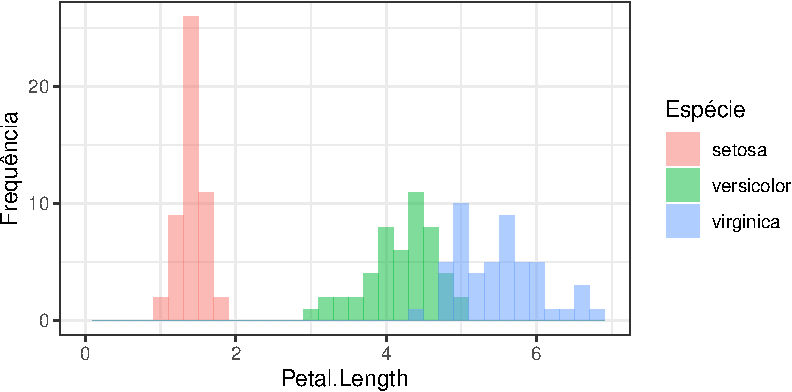
\includegraphics{lista-6_files/figure-pdf/fig-histogramairis-1.pdf}

}

\caption{\label{fig-histogramairis}Histograma de Petal Length do
conjunto de dados iris.}

\end{figure}%

~

Os histogramas na Figura~\ref{fig-histogramairis2} foram criados
manualmente com o mesmo binwidth, porém com origens variando entre
\(t_0 = 0\) e \(t_0 = 1\) para ilustrar a limitação da dependência deste
termo. Depreende-se portanto que está sendo usada a equação
\ref{eq:histograma}.

~

\begin{Shaded}
\begin{Highlighting}[]
\CommentTok{\# bindiwdth}
\NormalTok{bk1 }\OtherTok{\textless{}{-}} \FunctionTok{seq}\NormalTok{(}\FloatTok{0.5}\NormalTok{,}\FloatTok{7.1}\NormalTok{,}\AttributeTok{by =} \FloatTok{0.2}\NormalTok{)}
\NormalTok{bk2 }\OtherTok{\textless{}{-}} \FunctionTok{seq}\NormalTok{(}\DecValTok{1}\NormalTok{, }\DecValTok{7}\NormalTok{, }\AttributeTok{by =} \FloatTok{0.2}\NormalTok{)}

\FunctionTok{par}\NormalTok{(}\AttributeTok{mfrow =} \FunctionTok{c}\NormalTok{(}\DecValTok{1}\NormalTok{,}\DecValTok{2}\NormalTok{))}

\FunctionTok{hist}\NormalTok{(iris}\SpecialCharTok{$}\NormalTok{Petal.Length, }\AttributeTok{probability =}\NormalTok{ T, }\AttributeTok{breaks =}\NormalTok{ bk1,}
     \AttributeTok{ylim =} \FunctionTok{c}\NormalTok{(}\DecValTok{0}\NormalTok{,}\FloatTok{0.8}\NormalTok{), }\AttributeTok{col =} \StringTok{\textquotesingle{}blue\textquotesingle{}}\NormalTok{,}
     \AttributeTok{xlab =} \StringTok{\textquotesingle{}t0 = 0.5, h = 0.2\textquotesingle{}}\NormalTok{, }\AttributeTok{main =} \StringTok{""}\NormalTok{)}
\FunctionTok{rug}\NormalTok{(iris}\SpecialCharTok{$}\NormalTok{Petal.Length)}

\FunctionTok{hist}\NormalTok{(iris}\SpecialCharTok{$}\NormalTok{Petal.Length, }\AttributeTok{probability =}\NormalTok{ T, }\AttributeTok{breaks =}\NormalTok{ bk2,}
     \AttributeTok{ylim =} \FunctionTok{c}\NormalTok{(}\DecValTok{0}\NormalTok{,}\FloatTok{0.8}\NormalTok{), }\AttributeTok{col =} \StringTok{\textquotesingle{}blue\textquotesingle{}}\NormalTok{,}
     \AttributeTok{xlab =} \StringTok{\textquotesingle{}t0 = 1, h = 0.2\textquotesingle{}}\NormalTok{, }\AttributeTok{main =} \StringTok{""}\NormalTok{)}
\FunctionTok{rug}\NormalTok{(iris}\SpecialCharTok{$}\NormalTok{Petal.Length)}
\end{Highlighting}
\end{Shaded}

\begin{figure}[H]

\centering{

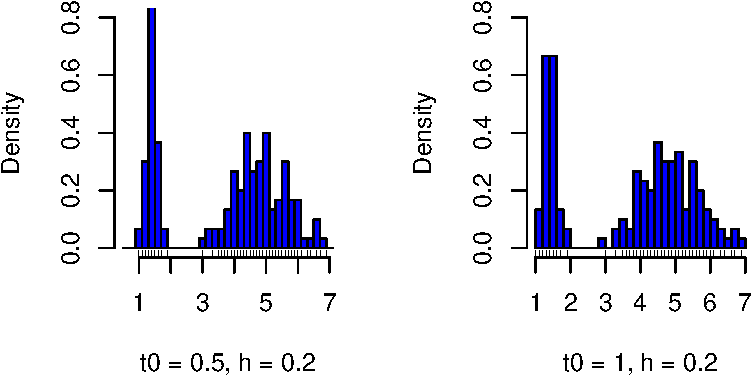
\includegraphics{lista-6_files/figure-pdf/fig-histogramairis2-1.pdf}

}

\caption{\label{fig-histogramairis2}Histograma manual de Petal Length do
conjunto de dados iris utilizando h = 0,2.}

\end{figure}%

~

Para a classificação, serão separados pontos de fronteira entre as
espécies. Esses mesmos pontos serão usados nos demais itens desta
questão.

~

\begin{Shaded}
\begin{Highlighting}[]
\CommentTok{\# iris com as variáveis selecionadas}
\NormalTok{iris2 }\OtherTok{\textless{}{-}}\NormalTok{ iris }\SpecialCharTok{\%\textgreater{}\%}\NormalTok{ dplyr}\SpecialCharTok{::}\FunctionTok{select}\NormalTok{(Petal.Length, Petal.Width, Species)}

\CommentTok{\# separação arbitrária de treino e teste}
\NormalTok{iris2 }\OtherTok{\textless{}{-}}\NormalTok{ iris2 }\SpecialCharTok{\%\textgreater{}\%}
  \FunctionTok{mutate}\NormalTok{(}\AttributeTok{partition =} \FunctionTok{case\_when}\NormalTok{(}
\NormalTok{    Petal.Length }\SpecialCharTok{==} \FloatTok{5.1} \SpecialCharTok{\&}\NormalTok{ Petal.Width }\SpecialCharTok{\%in\%} \FunctionTok{c}\NormalTok{(}\FloatTok{1.5}\NormalTok{, }\FloatTok{1.6}\NormalTok{) }\SpecialCharTok{\textasciitilde{}} \StringTok{"teste"}\NormalTok{,}
\NormalTok{    Petal.Length }\SpecialCharTok{==} \DecValTok{5} \SpecialCharTok{\&}\NormalTok{ Petal.Width }\SpecialCharTok{\%in\%} \FunctionTok{c}\NormalTok{(}\FloatTok{1.7}\NormalTok{, }\FloatTok{1.5}\NormalTok{) }\SpecialCharTok{\textasciitilde{}} \StringTok{"teste"}\NormalTok{,}
\NormalTok{    Petal.Length }\SpecialCharTok{==} \FloatTok{1.9} \SpecialCharTok{\&}\NormalTok{ Petal.Width }\SpecialCharTok{==} \FloatTok{0.4} \SpecialCharTok{\textasciitilde{}} \StringTok{"teste"}\NormalTok{,}
    \ConstantTok{TRUE} \SpecialCharTok{\textasciitilde{}} \StringTok{"treino"}
\NormalTok{  ))}
\end{Highlighting}
\end{Shaded}

~

Os histogramas para cada espécia são estimados a seguir:

~

\begin{Shaded}
\begin{Highlighting}[]
\CommentTok{\#setosa}
\NormalTok{hist\_setosa }\OtherTok{\textless{}{-}}\NormalTok{ iris2 }\SpecialCharTok{\%\textgreater{}\%}
\NormalTok{  dplyr}\SpecialCharTok{::}\FunctionTok{filter}\NormalTok{(Species }\SpecialCharTok{==} \StringTok{"setosa"}\NormalTok{, partition }\SpecialCharTok{==} \StringTok{"treino"}\NormalTok{) }\SpecialCharTok{\%$\%}
  \FunctionTok{hist}\NormalTok{(Petal.Length, }\AttributeTok{probability =}\NormalTok{ T, }\AttributeTok{breaks =}\NormalTok{ bk1)}
\end{Highlighting}
\end{Shaded}

\begin{Shaded}
\begin{Highlighting}[]
\CommentTok{\#virginica}
\NormalTok{hist\_virginica }\OtherTok{\textless{}{-}}\NormalTok{ iris2 }\SpecialCharTok{\%\textgreater{}\%}
\NormalTok{  dplyr}\SpecialCharTok{::}\FunctionTok{filter}\NormalTok{(Species }\SpecialCharTok{==} \StringTok{"virginica"}\NormalTok{, partition }\SpecialCharTok{==} \StringTok{"treino"}\NormalTok{) }\SpecialCharTok{\%$\%}
  \FunctionTok{hist}\NormalTok{(Petal.Length, }\AttributeTok{probability =}\NormalTok{ T, }\AttributeTok{breaks =}\NormalTok{ bk1)}
\end{Highlighting}
\end{Shaded}

\begin{Shaded}
\begin{Highlighting}[]
\CommentTok{\#versicolor}
\NormalTok{hist\_versicolor }\OtherTok{\textless{}{-}}\NormalTok{ iris2 }\SpecialCharTok{\%\textgreater{}\%}
\NormalTok{  dplyr}\SpecialCharTok{::}\FunctionTok{filter}\NormalTok{(Species }\SpecialCharTok{==} \StringTok{"versicolor"}\NormalTok{, partition }\SpecialCharTok{==} \StringTok{"treino"}\NormalTok{) }\SpecialCharTok{\%$\%}
  \FunctionTok{hist}\NormalTok{(Petal.Length, }\AttributeTok{probability =}\NormalTok{ T, }\AttributeTok{breaks =}\NormalTok{ bk1)}
\end{Highlighting}
\end{Shaded}

~

Finalmente, são acessados os resultados dos histogramas para construir a
Tabela~\ref{tbl-histogramasespecies} a seguir, em que apenas as
\emph{bins} com contagens superiores a zero são exibidas. As colunas da
tabela correspondem ao valor inicial de cada \emph{bin}, a contagem de
observações, a densidade e a espécie.

Pode-se observar que a espécie Setosa está em uma região de comprimento
de pétala bem separada das demais, então, para a classificação, basta
verificar se uma nova observação se encontra na mesma região que as
demais. Para as espécies Virginica e Versicolor, a separação não é tão
clara, então é necessário adotar uma regra. Como a densidade do
\emph{bin} com início em 4.5 é maior para Versicolor e o inverso ocorre
para o \emph{bin} com início em 4.7, a fronteira entre esses bins será a
regra de decisão. Isso implica em prováveis 2\% de erro de classificação
das Virgínica, quando se classifica em Versicolor, e 8.4\% de erro de
classificação das Versicolor, quando se classifica em
Virginica\footnote{Erros calculados a partir da sobreposição dos
  histogramas, considerando a fronteira de decisão.}.

~

\begin{Shaded}
\begin{Highlighting}[]
\FunctionTok{options}\NormalTok{(}\AttributeTok{knitr.kable.NA =} \StringTok{\textquotesingle{}{-}\textquotesingle{}}\NormalTok{)}

\CommentTok{\#monta a tabela com dados dos histogramas}
\FunctionTok{tibble}\NormalTok{(}
  \AttributeTok{ti =}\NormalTok{ hist\_setosa}\SpecialCharTok{$}\NormalTok{breaks[}\SpecialCharTok{{-}}\DecValTok{34}\NormalTok{],}
  \AttributeTok{cont.setosa =}\NormalTok{ hist\_setosa}\SpecialCharTok{$}\NormalTok{counts,}
  \AttributeTok{dens.setosa =}\NormalTok{ hist\_setosa}\SpecialCharTok{$}\NormalTok{density,}
  \AttributeTok{cont.virginica =}\NormalTok{ hist\_virginica}\SpecialCharTok{$}\NormalTok{counts,}
  \AttributeTok{dens.virginica =}\NormalTok{ hist\_virginica}\SpecialCharTok{$}\NormalTok{density,}
  \AttributeTok{cont.versicolor =}\NormalTok{ hist\_versicolor}\SpecialCharTok{$}\NormalTok{counts,}
  \AttributeTok{dens.versicolor =}\NormalTok{ hist\_versicolor}\SpecialCharTok{$}\NormalTok{density}
\NormalTok{) }\SpecialCharTok{\%\textgreater{}\%}
  \CommentTok{\# seleciona linhas com valores maiores que zero}
\NormalTok{  dplyr}\SpecialCharTok{::}\FunctionTok{filter}\NormalTok{(}\FunctionTok{if\_any}\NormalTok{(}\SpecialCharTok{{-}}\NormalTok{ti, }\SpecialCharTok{\textasciitilde{}}\NormalTok{ . }\SpecialCharTok{\textgreater{}} \DecValTok{0}\NormalTok{)) }\SpecialCharTok{\%\textgreater{}\%}
  \CommentTok{\# ajusta decimais para arrumar o tamanho da tabela}
  \FunctionTok{mutate}\NormalTok{(}\FunctionTok{across}\NormalTok{(}\FunctionTok{everything}\NormalTok{(), }\SpecialCharTok{\textasciitilde{}} \FunctionTok{round}\NormalTok{(., }\DecValTok{2}\NormalTok{)),}
         \FunctionTok{across}\NormalTok{(}\FunctionTok{everything}\NormalTok{(), }\SpecialCharTok{\textasciitilde{}} \FunctionTok{if\_else}\NormalTok{(. }\SpecialCharTok{==} \DecValTok{0}\NormalTok{, }\ConstantTok{NA}\NormalTok{, .))) }\SpecialCharTok{\%\textgreater{}\%} 
  \CommentTok{\# gera tabela tex}
\NormalTok{  knitr}\SpecialCharTok{::}\FunctionTok{kable}\NormalTok{(}
    \AttributeTok{align =} \StringTok{"c"}
\NormalTok{  )}
\end{Highlighting}
\end{Shaded}

\begin{longtable}[]{@{}
  >{\centering\arraybackslash}p{(\columnwidth - 12\tabcolsep) * \real{0.0515}}
  >{\centering\arraybackslash}p{(\columnwidth - 12\tabcolsep) * \real{0.1340}}
  >{\centering\arraybackslash}p{(\columnwidth - 12\tabcolsep) * \real{0.1340}}
  >{\centering\arraybackslash}p{(\columnwidth - 12\tabcolsep) * \real{0.1649}}
  >{\centering\arraybackslash}p{(\columnwidth - 12\tabcolsep) * \real{0.1649}}
  >{\centering\arraybackslash}p{(\columnwidth - 12\tabcolsep) * \real{0.1753}}
  >{\centering\arraybackslash}p{(\columnwidth - 12\tabcolsep) * \real{0.1753}}@{}}

\caption{\label{tbl-histogramasespecies}Histogramas de Petal Length do
conjunto de dados iris.}

\tabularnewline

\toprule\noalign{}
\begin{minipage}[b]{\linewidth}\centering
ti
\end{minipage} & \begin{minipage}[b]{\linewidth}\centering
cont.setosa
\end{minipage} & \begin{minipage}[b]{\linewidth}\centering
dens.setosa
\end{minipage} & \begin{minipage}[b]{\linewidth}\centering
cont.virginica
\end{minipage} & \begin{minipage}[b]{\linewidth}\centering
dens.virginica
\end{minipage} & \begin{minipage}[b]{\linewidth}\centering
cont.versicolor
\end{minipage} & \begin{minipage}[b]{\linewidth}\centering
dens.versicolor
\end{minipage} \\
\midrule\noalign{}
\endhead
\bottomrule\noalign{}
\endlastfoot
0.9 & 2 & 0.20 & - & - & - & - \\
1.1 & 9 & 0.92 & - & - & - & - \\
1.3 & 26 & 2.65 & - & - & - & - \\
1.5 & 11 & 1.12 & - & - & - & - \\
1.7 & 1 & 0.10 & - & - & - & - \\
2.9 & - & - & - & - & 1 & 0.10 \\
3.1 & - & - & - & - & 2 & 0.21 \\
3.3 & - & - & - & - & 2 & 0.21 \\
3.5 & - & - & - & - & 2 & 0.21 \\
3.7 & - & - & - & - & 4 & 0.42 \\
3.9 & - & - & - & - & 8 & 0.83 \\
4.1 & - & - & - & - & 6 & 0.62 \\
4.3 & - & - & 1 & 0.10 & 11 & 1.15 \\
4.5 & - & - & - & - & 8 & 0.83 \\
4.7 & - & - & 5 & 0.52 & 4 & 0.42 \\
4.9 & - & - & 8 & 0.83 & - & - \\
5.1 & - & - & 4 & 0.42 & - & - \\
5.3 & - & - & 5 & 0.52 & - & - \\
5.5 & - & - & 9 & 0.94 & - & - \\
5.7 & - & - & 5 & 0.52 & - & - \\
5.9 & - & - & 5 & 0.52 & - & - \\
6.1 & - & - & 1 & 0.10 & - & - \\
6.3 & - & - & 1 & 0.10 & - & - \\
6.5 & - & - & 3 & 0.31 & - & - \\
6.7 & - & - & 1 & 0.10 & - & - \\

\end{longtable}

~

Em posse das regras de decisão, classifica-se os pontos de teste e se
obtém a Tabela~\ref{tbl-histogramasespecies2} a seguir.

~

\begin{Shaded}
\begin{Highlighting}[]
\NormalTok{iris2 }\SpecialCharTok{\%\textgreater{}\%}
\NormalTok{  dplyr}\SpecialCharTok{::}\FunctionTok{filter}\NormalTok{(partition }\SpecialCharTok{==} \StringTok{"teste"}\NormalTok{) }\SpecialCharTok{\%\textgreater{}\%}
\NormalTok{  dplyr}\SpecialCharTok{::}\FunctionTok{select}\NormalTok{(}\SpecialCharTok{{-}}\NormalTok{Petal.Width, }\SpecialCharTok{{-}}\NormalTok{partition) }\SpecialCharTok{\%\textgreater{}\%}
  \FunctionTok{mutate}\NormalTok{(}\StringTok{\textasciigrave{}}\AttributeTok{Classificação}\StringTok{\textasciigrave{}} \OtherTok{=} \FunctionTok{c}\NormalTok{(}\StringTok{"setosa"}\NormalTok{, }\FunctionTok{rep}\NormalTok{(}\StringTok{"virginica"}\NormalTok{, }\DecValTok{4}\NormalTok{))) }\SpecialCharTok{\%\textgreater{}\%}
\NormalTok{  knitr}\SpecialCharTok{::}\FunctionTok{kable}\NormalTok{(}\AttributeTok{align =} \StringTok{"cll"}\NormalTok{)}
\end{Highlighting}
\end{Shaded}

\begin{longtable}[]{@{}cll@{}}

\caption{\label{tbl-histogramasespecies2}Classificação dos pontos de
teste do conjunto de dados iris via histograma.}

\tabularnewline

\toprule\noalign{}
Petal.Length & Species & Classificação \\
\midrule\noalign{}
\endhead
\bottomrule\noalign{}
\endlastfoot
1.9 & setosa & setosa \\
5.0 & versicolor & virginica \\
5.1 & versicolor & virginica \\
5.0 & virginica & virginica \\
5.1 & virginica & virginica \\

\end{longtable}

~

\subsection{Estimação baseada em
Núcleos}\label{estimauxe7uxe3o-baseada-em-nuxfacleos}

Soliciona outro problema do Método do Histograma, que é a necessidade de
se utilizar intervalos pequenos e \(n\) grande para se obter uma boa
aproximação da densidade alvo. O estimador de densidade no caso
univariado é dado por

\[
\hat{f}(x; h) = \frac{1}{n} \sum_{i=1}^n k \,h(x - X_i),
\] ~

enquanto no caso multivariado é dado por

\[
\hat{f}(x; h) = \frac{1}{n |\mathbf{H}|^{1/2}} \sum_{i=1}^n k(\mathbf{H}^{-1/2}(\mathbf{x} - \mathbf{X}_i)).
\] ~

Nas expressões \(k\) é o núcleo de uma função densidade arbitrária. Um
problema que surge é a seleção do bandwidth \(h\), que será demonstrado
a seguir utilizando o pacote \texttt{ks} para a obtenção da matriz
\(\mathbf{H}_{p\times p}\) de intervalos\footnote{Para o caso
  unidimensional, i.e.~\(p = 1\), \(\mathbf{H} = h^2\).}.

A seguir é estimada a densidade conjunta para as variáveis
\texttt{Petal.Length} e \texttt{Petal.Width} com o conjunto de teste,
seguida da Figura~\ref{fig-kdeiris} ilustrando-a. Os pontos de cor azul
correspondem aos pontos de teste.

~

\begin{Shaded}
\begin{Highlighting}[]
\CommentTok{\# obtenção da matriz H}
\NormalTok{He }\OtherTok{\textless{}{-}}\NormalTok{ iris2 }\SpecialCharTok{\%\textgreater{}\%} 
\NormalTok{  dplyr}\SpecialCharTok{::}\FunctionTok{filter}\NormalTok{(partition }\SpecialCharTok{==} \StringTok{"treino"}\NormalTok{) }\SpecialCharTok{\%\textgreater{}\%}
\NormalTok{  dplyr}\SpecialCharTok{::}\FunctionTok{select}\NormalTok{(Petal.Length, Petal.Width) }\SpecialCharTok{\%\textgreater{}\%}
\NormalTok{  ks}\SpecialCharTok{::}\FunctionTok{Hpi}\NormalTok{()}

\CommentTok{\# kernel density estimation com a H estimada}
\NormalTok{kdeHe }\OtherTok{\textless{}{-}}\NormalTok{ iris2 }\SpecialCharTok{\%\textgreater{}\%} 
\NormalTok{  dplyr}\SpecialCharTok{::}\FunctionTok{filter}\NormalTok{(partition }\SpecialCharTok{==} \StringTok{"treino"}\NormalTok{) }\SpecialCharTok{\%\textgreater{}\%}
\NormalTok{  dplyr}\SpecialCharTok{::}\FunctionTok{select}\NormalTok{(Petal.Length, Petal.Width) }\SpecialCharTok{\%\textgreater{}\%}
\NormalTok{  ks}\SpecialCharTok{::}\FunctionTok{kde}\NormalTok{(., }\AttributeTok{H=}\NormalTok{He)}
\end{Highlighting}
\end{Shaded}

~

\begin{Shaded}
\begin{Highlighting}[]
\NormalTok{pteste }\OtherTok{\textless{}{-}}\NormalTok{ iris2 }\SpecialCharTok{\%\textgreater{}\%}
\NormalTok{  dplyr}\SpecialCharTok{::}\FunctionTok{filter}\NormalTok{(partition }\SpecialCharTok{==} \StringTok{"teste"}\NormalTok{) }\SpecialCharTok{\%\textgreater{}\%}
\NormalTok{  dplyr}\SpecialCharTok{::}\FunctionTok{select}\NormalTok{(Petal.Length, Petal.Width) }\SpecialCharTok{\%\textgreater{}\%}
  \FunctionTok{as.matrix}\NormalTok{()}

\FunctionTok{par}\NormalTok{(}\AttributeTok{mar =} \FunctionTok{c}\NormalTok{(}\DecValTok{3}\NormalTok{,}\DecValTok{4}\NormalTok{,}\DecValTok{4}\NormalTok{,}\DecValTok{4}\NormalTok{), }\AttributeTok{pin =} \FunctionTok{c}\NormalTok{(}\DecValTok{4}\NormalTok{, }\FloatTok{2.75}\NormalTok{))}

\FunctionTok{image}\NormalTok{(kdeHe}\SpecialCharTok{$}\NormalTok{eval.points[[}\DecValTok{1}\NormalTok{]],kdeHe}\SpecialCharTok{$}\NormalTok{eval.points[[}\DecValTok{2}\NormalTok{]],}
\NormalTok{      kdeHe}\SpecialCharTok{$}\NormalTok{estimate, }\AttributeTok{xlab =} \StringTok{\textquotesingle{}Petal Length\textquotesingle{}}\NormalTok{,}
      \AttributeTok{ylab =} \StringTok{\textquotesingle{}Petal Width\textquotesingle{}}\NormalTok{)}
\FunctionTok{points}\NormalTok{(kdeHe}\SpecialCharTok{$}\NormalTok{x, }\AttributeTok{col =} \FunctionTok{alpha}\NormalTok{(}\StringTok{"black"}\NormalTok{, }\FloatTok{0.3}\NormalTok{))}
\FunctionTok{points}\NormalTok{(pteste, }\AttributeTok{col =} \StringTok{"blue"}\NormalTok{, }\AttributeTok{pch =} \DecValTok{8}\NormalTok{)}
\end{Highlighting}
\end{Shaded}

\begin{figure}[H]

\centering{

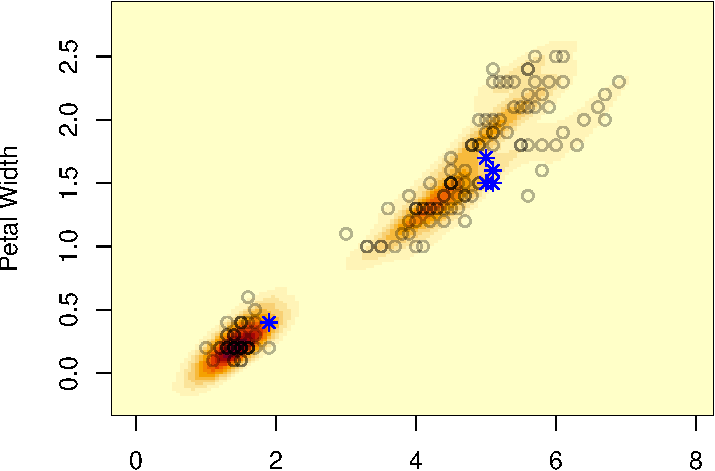
\includegraphics{lista-6_files/figure-pdf/fig-kdeiris-1.pdf}

}

\caption{\label{fig-kdeiris}Densidade estimada do conjunto de dados de
treino iris para comprimento e largura da pétala.}

\end{figure}%

Como a classificação da espécia Setosa é novamente óbvia, apenas a
classificação para as demais espécies será feita. As densidades para
Virgínica e Versicolor são estimadas a seguir.

~

\begin{Shaded}
\begin{Highlighting}[]
\CommentTok{\# H versicolor}
\NormalTok{He\_versi }\OtherTok{\textless{}{-}}\NormalTok{ iris2 }\SpecialCharTok{\%\textgreater{}\%} 
\NormalTok{  dplyr}\SpecialCharTok{::}\FunctionTok{filter}\NormalTok{(partition }\SpecialCharTok{==} \StringTok{"treino"}\NormalTok{, Species }\SpecialCharTok{==} \StringTok{"versicolor"}\NormalTok{) }\SpecialCharTok{\%\textgreater{}\%}
\NormalTok{  dplyr}\SpecialCharTok{::}\FunctionTok{select}\NormalTok{(Petal.Length, Petal.Width) }\SpecialCharTok{\%\textgreater{}\%}
\NormalTok{  ks}\SpecialCharTok{::}\FunctionTok{Hpi}\NormalTok{()}

\CommentTok{\# kde versi}
\NormalTok{kdeHe\_versi }\OtherTok{\textless{}{-}}\NormalTok{ iris2 }\SpecialCharTok{\%\textgreater{}\%} 
\NormalTok{  dplyr}\SpecialCharTok{::}\FunctionTok{filter}\NormalTok{(partition }\SpecialCharTok{==} \StringTok{"treino"}\NormalTok{, Species }\SpecialCharTok{==} \StringTok{"versicolor"}\NormalTok{) }\SpecialCharTok{\%\textgreater{}\%}
\NormalTok{  dplyr}\SpecialCharTok{::}\FunctionTok{select}\NormalTok{(Petal.Length, Petal.Width) }\SpecialCharTok{\%\textgreater{}\%}
\NormalTok{  ks}\SpecialCharTok{::}\FunctionTok{kde}\NormalTok{(., }\AttributeTok{H=}\NormalTok{He\_versi)}

\CommentTok{\# H virginica}
\NormalTok{He\_virg }\OtherTok{\textless{}{-}}\NormalTok{ iris2 }\SpecialCharTok{\%\textgreater{}\%} 
\NormalTok{  dplyr}\SpecialCharTok{::}\FunctionTok{filter}\NormalTok{(partition }\SpecialCharTok{==} \StringTok{"treino"}\NormalTok{, Species }\SpecialCharTok{==} \StringTok{"virginica"}\NormalTok{) }\SpecialCharTok{\%\textgreater{}\%}
\NormalTok{  dplyr}\SpecialCharTok{::}\FunctionTok{select}\NormalTok{(Petal.Length, Petal.Width) }\SpecialCharTok{\%\textgreater{}\%}
\NormalTok{  ks}\SpecialCharTok{::}\FunctionTok{Hpi}\NormalTok{()}

\CommentTok{\# kde virginica}
\NormalTok{kdeHe\_virg }\OtherTok{\textless{}{-}}\NormalTok{ iris2 }\SpecialCharTok{\%\textgreater{}\%} 
\NormalTok{  dplyr}\SpecialCharTok{::}\FunctionTok{filter}\NormalTok{(partition }\SpecialCharTok{==} \StringTok{"treino"}\NormalTok{, Species }\SpecialCharTok{==} \StringTok{"virginica"}\NormalTok{) }\SpecialCharTok{\%\textgreater{}\%}
\NormalTok{  dplyr}\SpecialCharTok{::}\FunctionTok{select}\NormalTok{(Petal.Length, Petal.Width) }\SpecialCharTok{\%\textgreater{}\%}
\NormalTok{  ks}\SpecialCharTok{::}\FunctionTok{kde}\NormalTok{(., }\AttributeTok{H=}\NormalTok{He\_virg)}
\end{Highlighting}
\end{Shaded}

~

Os valores das densidades para os pontos de teste são dados na
Tabela~\ref{tbl-classificakde} a seguir, assim como as suas
classificações.

~

\begin{Shaded}
\begin{Highlighting}[]
\NormalTok{pteste2 }\OtherTok{\textless{}{-}}\NormalTok{ iris2 }\SpecialCharTok{\%\textgreater{}\%} 
\NormalTok{  dplyr}\SpecialCharTok{::}\FunctionTok{filter}\NormalTok{(partition }\SpecialCharTok{==} \StringTok{"teste"}\NormalTok{, Species }\SpecialCharTok{!=} \StringTok{"setosa"}\NormalTok{) }\SpecialCharTok{\%\textgreater{}\%}
\NormalTok{  dplyr}\SpecialCharTok{::}\FunctionTok{select}\NormalTok{(Petal.Length, Petal.Width) }\SpecialCharTok{\%\textgreater{}\%}
  \FunctionTok{as.matrix}\NormalTok{()}

\NormalTok{iris2 }\SpecialCharTok{\%\textgreater{}\%} 
\NormalTok{  dplyr}\SpecialCharTok{::}\FunctionTok{filter}\NormalTok{(partition }\SpecialCharTok{==} \StringTok{"teste"}\NormalTok{, Species }\SpecialCharTok{!=} \StringTok{"setosa"}\NormalTok{) }\SpecialCharTok{\%\textgreater{}\%}
\NormalTok{  dplyr}\SpecialCharTok{::}\FunctionTok{select}\NormalTok{(Petal.Length, Petal.Width, Species) }\SpecialCharTok{\%\textgreater{}\%}
  \FunctionTok{mutate}\NormalTok{(}\AttributeTok{dens.versi =} \FunctionTok{predict}\NormalTok{(kdeHe\_versi, }\AttributeTok{x =}\NormalTok{ pteste2),}
         \AttributeTok{dens.virg =} \FunctionTok{predict}\NormalTok{(kdeHe\_virg, }\AttributeTok{x =}\NormalTok{ pteste2),}
         \StringTok{\textasciigrave{}}\AttributeTok{Classificação}\StringTok{\textasciigrave{}} \OtherTok{=} \FunctionTok{if\_else}\NormalTok{(dens.versi }\SpecialCharTok{\textgreater{}}\NormalTok{ dens.virg, }\StringTok{"versicolor"}\NormalTok{, }\StringTok{"virginica"}\NormalTok{)) }\SpecialCharTok{\%\textgreater{}\%}
\NormalTok{  knitr}\SpecialCharTok{::}\FunctionTok{kable}\NormalTok{(}\AttributeTok{align =} \StringTok{"cclccl"}\NormalTok{,}
               \AttributeTok{digits =} \DecValTok{2}\NormalTok{)}
\end{Highlighting}
\end{Shaded}

\begin{longtable}[]{@{}
  >{\centering\arraybackslash}p{(\columnwidth - 10\tabcolsep) * \real{0.1867}}
  >{\centering\arraybackslash}p{(\columnwidth - 10\tabcolsep) * \real{0.1733}}
  >{\raggedright\arraybackslash}p{(\columnwidth - 10\tabcolsep) * \real{0.1467}}
  >{\centering\arraybackslash}p{(\columnwidth - 10\tabcolsep) * \real{0.1600}}
  >{\centering\arraybackslash}p{(\columnwidth - 10\tabcolsep) * \real{0.1467}}
  >{\raggedright\arraybackslash}p{(\columnwidth - 10\tabcolsep) * \real{0.1867}}@{}}

\caption{\label{tbl-classificakde}Classificação dos pontos de teste com
densidades estimadas para Virgínica e Versicolor.}

\tabularnewline

\toprule\noalign{}
\begin{minipage}[b]{\linewidth}\centering
Petal.Length
\end{minipage} & \begin{minipage}[b]{\linewidth}\centering
Petal.Width
\end{minipage} & \begin{minipage}[b]{\linewidth}\raggedright
Species
\end{minipage} & \begin{minipage}[b]{\linewidth}\centering
dens.versi
\end{minipage} & \begin{minipage}[b]{\linewidth}\centering
dens.virg
\end{minipage} & \begin{minipage}[b]{\linewidth}\raggedright
Classificação
\end{minipage} \\
\midrule\noalign{}
\endhead
\bottomrule\noalign{}
\endlastfoot
5.0 & 1.7 & versicolor & 0.27 & 0.46 & virginica \\
5.1 & 1.6 & versicolor & 0.45 & 0.15 & versicolor \\
5.0 & 1.5 & virginica & 0.84 & 0.04 & versicolor \\
5.1 & 1.5 & virginica & 0.42 & 0.04 & versicolor \\

\end{longtable}

~

\subsection{k-Vizinhos mais Próximos
(KNN)}\label{k-vizinhos-mais-pruxf3ximos-knn}

O método de k-vizinhos mais próximos (\(k\) \emph{nearest neighbors})
pretende classificar um determinado ponto \(\mathbf{x}_0\) a partir dos
\(k\) pontos mais próximos. A classificação é dada em função da menor
distância euclidiana entre \(\mathbf{x}_0\) e os pontos de treinamento
e, se houver empate, a escolha é feita aleatoriamente. Enquanto há
muitas medidas de distância possíveis, a mais comum é a distância
euclidiana, dada por

\[
d(\mathbf{x}_i, \mathbf{x}_0) = \sqrt{ \sum_{l=1}^p (x_{il} - x_{0l})^2 } = ||\mathbf{x}_i - \mathbf{x}_0||_2.
\] ~

A Figura~\ref{fig-scatteriris2} apresenta um gráfico de dispersão do
conjunto de dados em função das variáveis de interesse, no qual as cores
indicam a espécie e as formas indicam a partição de treino ou teste. As
unidades de teste foram selecionadas de forma arbitrária visando
ilustrar as limitações desse método.

Enquanto é esperado que o ponto de teste de espécie Setosa seja
classificado corretamente, não se pode esperar uma classificação correta
dos pontos de teste de espécie Versicolor e Virginica, visto que estão
numa fronteira difusa entre os grupos.

~

\begin{Shaded}
\begin{Highlighting}[]
\CommentTok{\# gráfico}
\FunctionTok{ggplot}\NormalTok{() }\SpecialCharTok{+}
  \FunctionTok{geom\_point}\NormalTok{(}\AttributeTok{data =}\NormalTok{ iris2[iris2}\SpecialCharTok{$}\NormalTok{partition }\SpecialCharTok{==} \StringTok{"teste"}\NormalTok{,], }\FunctionTok{aes}\NormalTok{(}\AttributeTok{x =}\NormalTok{ Petal.Length, }\AttributeTok{y =}\NormalTok{ Petal.Width, }\AttributeTok{color =}\NormalTok{ Species), }\AttributeTok{shape =} \DecValTok{8}\NormalTok{) }\SpecialCharTok{+}
  \FunctionTok{geom\_point}\NormalTok{(}\AttributeTok{data =}\NormalTok{ iris2[iris2}\SpecialCharTok{$}\NormalTok{partition }\SpecialCharTok{==} \StringTok{"treino"}\NormalTok{,], }\FunctionTok{aes}\NormalTok{(}\AttributeTok{x =}\NormalTok{ Petal.Length, }\AttributeTok{y =}\NormalTok{ Petal.Width, }\AttributeTok{color =}\NormalTok{ Species), }\AttributeTok{shape =} \DecValTok{16}\NormalTok{) }\SpecialCharTok{+}
  \FunctionTok{theme\_bw}\NormalTok{() }\SpecialCharTok{+}
  \FunctionTok{labs}\NormalTok{(}\AttributeTok{x =} \StringTok{"Petal.Length"}\NormalTok{,}
    \AttributeTok{y =} \StringTok{"Petal.Width"}\NormalTok{,}
    \AttributeTok{color =} \StringTok{"Espécie"}\NormalTok{,}
    \AttributeTok{shape =} \StringTok{"Partição"}\NormalTok{)}
\end{Highlighting}
\end{Shaded}

\begin{figure}[H]

\centering{

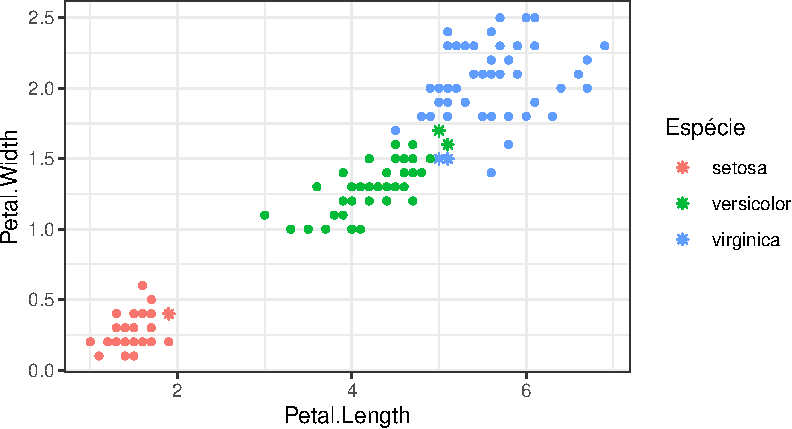
\includegraphics{lista-6_files/figure-pdf/fig-scatteriris2-1.pdf}

}

\caption{\label{fig-scatteriris2}Gráfico de dispersão do conjunto de
dados iris.}

\end{figure}%

~

A Tabela~\ref{tbl-knniris} apresenta a espécie real dos pontos de teste,
bem como a classificação utilizando os 3 e cinco vizinhos mais próximos
(knn = 3 e knn = 5 respectivamente). O comportamento é exatamente o
esperado.

~

\begin{Shaded}
\begin{Highlighting}[]
\NormalTok{treino }\OtherTok{\textless{}{-}}\NormalTok{ iris2 }\SpecialCharTok{\%\textgreater{}\%} \FunctionTok{filter}\NormalTok{(partition }\SpecialCharTok{==} \StringTok{"treino"}\NormalTok{)}
\NormalTok{teste }\OtherTok{\textless{}{-}}\NormalTok{ iris2 }\SpecialCharTok{\%\textgreater{}\%} \FunctionTok{filter}\NormalTok{(partition }\SpecialCharTok{==} \StringTok{"teste"}\NormalTok{)}

\NormalTok{knn3 }\OtherTok{\textless{}{-}} \FunctionTok{knn}\NormalTok{(}\AttributeTok{train =}\NormalTok{ treino[, }\FunctionTok{c}\NormalTok{(}\DecValTok{1}\NormalTok{,}\DecValTok{2}\NormalTok{)],}
    \AttributeTok{test =}\NormalTok{ teste[, }\FunctionTok{c}\NormalTok{(}\DecValTok{1}\NormalTok{,}\DecValTok{2}\NormalTok{)],}
    \AttributeTok{cl =}\NormalTok{ treino}\SpecialCharTok{$}\NormalTok{Species,}
    \AttributeTok{k =} \DecValTok{3}\NormalTok{)}

\NormalTok{knn5 }\OtherTok{\textless{}{-}} \FunctionTok{knn}\NormalTok{(}\AttributeTok{train =}\NormalTok{ treino[, }\FunctionTok{c}\NormalTok{(}\DecValTok{1}\NormalTok{,}\DecValTok{2}\NormalTok{)],}
    \AttributeTok{test =}\NormalTok{ teste[, }\FunctionTok{c}\NormalTok{(}\DecValTok{1}\NormalTok{,}\DecValTok{2}\NormalTok{)],}
    \AttributeTok{cl =}\NormalTok{ treino}\SpecialCharTok{$}\NormalTok{Species,}
    \AttributeTok{k =} \DecValTok{5}\NormalTok{)}

\FunctionTok{data.frame}\NormalTok{(}
\NormalTok{  teste}\SpecialCharTok{$}\NormalTok{Species,}
\NormalTok{  knn3,}
\NormalTok{  knn5}
\NormalTok{) }\SpecialCharTok{\%\textgreater{}\%}
\NormalTok{  knitr}\SpecialCharTok{::}\FunctionTok{kable}\NormalTok{(}
    \AttributeTok{col.names =} \FunctionTok{c}\NormalTok{(}\StringTok{"Espécie real"}\NormalTok{, }\StringTok{"k = 3"}\NormalTok{, }\StringTok{"k = 5"}\NormalTok{)}
\NormalTok{  )}
\end{Highlighting}
\end{Shaded}

\begin{longtable}[]{@{}lll@{}}

\caption{\label{tbl-knniris}Classificação dos pontos de teste do
conjunto de dados iris.}

\tabularnewline

\toprule\noalign{}
Espécie real & k = 3 & k = 5 \\
\midrule\noalign{}
\endhead
\bottomrule\noalign{}
\endlastfoot
setosa & setosa & setosa \\
versicolor & virginica & virginica \\
versicolor & versicolor & virginica \\
virginica & versicolor & versicolor \\
virginica & versicolor & virginica \\

\end{longtable}

~

Finalmente, projeta-se a classificação dos pontos de acordo com os dois
algoritmos KNN utilizados na Figura~\ref{fig-knniris}. O conjunto
completo é exibido no gráfico central da segunda linha.

~

\begin{figure}[H]

\centering{

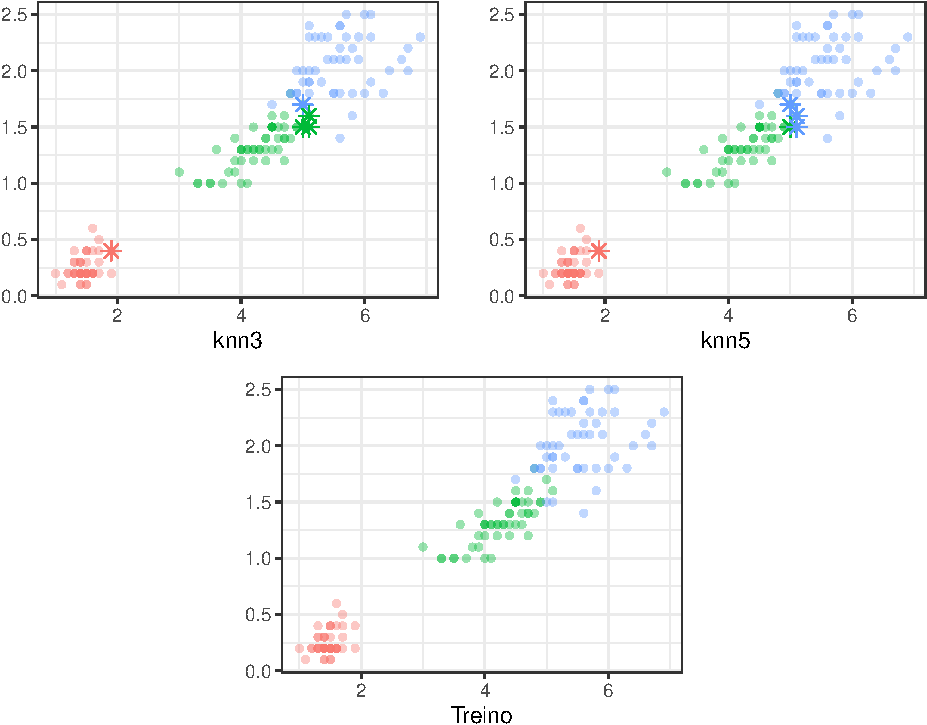
\includegraphics{lista-6_files/figure-pdf/fig-knniris-1.pdf}

}

\caption{\label{fig-knniris}Classificação dos pontos de teste do
conjunto de dados iris.}

\end{figure}%

~

\section{Questão 16}\label{questuxe3o-16}

Estudar o pacote \texttt{ks} do R e apresentar um exemplo.

\begin{center}\rule{0.5\linewidth}{0.5pt}\end{center}

~

~

\section{Questão 17}\label{questuxe3o-17}

Apresentar um exemplo com classificador LDA e QDA.

\begin{center}\rule{0.5\linewidth}{0.5pt}\end{center}

Como auxiliar, será definido um método \texttt{is\_cov}, para garantir
que as matrizes de variância-covariância (que serão geradas
aleatoriamente) satisfazem as condições necessárias. Será definida
também uma função que calcula a acurácia de um modelo.

\begin{Shaded}
\begin{Highlighting}[]
\NormalTok{is\_cov }\OtherTok{\textless{}{-}} \ControlFlowTok{function}\NormalTok{(Sigma) \{}

\NormalTok{  is\_square }\OtherTok{\textless{}{-}} \FunctionTok{nrow}\NormalTok{(Sigma) }\SpecialCharTok{==} \FunctionTok{ncol}\NormalTok{(Sigma)}
  
\NormalTok{  is\_symmetric }\OtherTok{\textless{}{-}} \FunctionTok{all}\NormalTok{(}\FunctionTok{t}\NormalTok{(Sigma) }\SpecialCharTok{==}\NormalTok{ Sigma)}
  
\NormalTok{  positive\_diag }\OtherTok{\textless{}{-}} \FunctionTok{all}\NormalTok{(}\FunctionTok{diag}\NormalTok{(Sigma) }\SpecialCharTok{\textgreater{}} \DecValTok{0}\NormalTok{)}
  
\NormalTok{  eigen\_greater\_zero }\OtherTok{\textless{}{-}} \FunctionTok{all}\NormalTok{(}\FunctionTok{with}\NormalTok{(}\FunctionTok{eigen}\NormalTok{(Sigma), values) }\SpecialCharTok{\textgreater{}} \DecValTok{0}\NormalTok{)}
  
\NormalTok{  cov\_smaller\_than\_sds }\OtherTok{\textless{}{-}} \ConstantTok{TRUE}

  \ControlFlowTok{for}\NormalTok{ (row }\ControlFlowTok{in} \DecValTok{1}\SpecialCharTok{:}\NormalTok{p) \{}
    \ControlFlowTok{for}\NormalTok{ (col }\ControlFlowTok{in}\NormalTok{ row}\SpecialCharTok{:}\NormalTok{p) \{}
\NormalTok{      cov\_smaller\_than\_sds }\OtherTok{\textless{}{-}}\NormalTok{ cov\_smaller\_than\_sds }\SpecialCharTok{\&}\NormalTok{ (}
        \FunctionTok{abs}\NormalTok{(Sigma[row, col]) }\SpecialCharTok{\textless{}=} \FunctionTok{sqrt}\NormalTok{(Sigma[row, row] }\SpecialCharTok{*}\NormalTok{ Sigma[col, col])}
\NormalTok{      )}
\NormalTok{    \}}
\NormalTok{  \}}

  \FunctionTok{all}\NormalTok{(}
\NormalTok{    is\_square, is\_symmetric, positive\_diag,}
\NormalTok{    cov\_smaller\_than\_sds, eigen\_greater\_zero}
\NormalTok{  )}
\NormalTok{\}}

\NormalTok{accuracy }\OtherTok{\textless{}{-}} \ControlFlowTok{function}\NormalTok{(model, data, response) \{}
\NormalTok{  prediction }\OtherTok{\textless{}{-}} \FunctionTok{predict}\NormalTok{(model, data)}\SpecialCharTok{$}\NormalTok{class }

  \FunctionTok{round}\NormalTok{(}\FunctionTok{sum}\NormalTok{(prediction }\SpecialCharTok{==}\NormalTok{ response) }\SpecialCharTok{/} \FunctionTok{length}\NormalTok{(response), }\DecValTok{3}\NormalTok{)}
\NormalTok{\}}
\end{Highlighting}
\end{Shaded}

Em seguida, será criada uma matriz de variâncias-covariâncias, a partir
da qual será criada uma normal multivariada. Essa matriz será
multiplicada pela sua transposta, de modo que satisfaça as condições
necessárias para ser uma matriz de variância-covariância.

~

\begin{Shaded}
\begin{Highlighting}[]
\NormalTok{p }\OtherTok{\textless{}{-}} \DecValTok{3}

\FunctionTok{set.seed}\NormalTok{(}\FunctionTok{exp}\NormalTok{(}\DecValTok{1}\NormalTok{))}

\NormalTok{Sigma }\OtherTok{\textless{}{-}} \FunctionTok{rnorm}\NormalTok{(p }\SpecialCharTok{\^{}} \DecValTok{2}\NormalTok{) }\SpecialCharTok{\%\textgreater{}\%}
    \FunctionTok{matrix}\NormalTok{(p, p) }\SpecialCharTok{\%\textgreater{}\%}
\NormalTok{    (}\ControlFlowTok{function}\NormalTok{(mat) }\FunctionTok{t}\NormalTok{(mat) }\SpecialCharTok{\%*\%}\NormalTok{ mat)}

\FunctionTok{round}\NormalTok{(Sigma, }\DecValTok{3}\NormalTok{)}
\end{Highlighting}
\end{Shaded}

\begin{verbatim}
      [,1]   [,2]   [,3]
[1,] 3.360  1.209  2.472
[2,] 1.209  1.302 -0.518
[3,] 2.472 -0.518  4.497
\end{verbatim}

\begin{Shaded}
\begin{Highlighting}[]
\FunctionTok{is\_cov}\NormalTok{(Sigma)}
\end{Highlighting}
\end{Shaded}

\begin{verbatim}
[1] TRUE
\end{verbatim}

~

Criando os dados, com mesma variância e vetores de média diferentes
(também gerados aleatoriamente), teremos:

~

\begin{Shaded}
\begin{Highlighting}[]
\NormalTok{muA }\OtherTok{\textless{}{-}} \FunctionTok{rnorm}\NormalTok{(p, }\AttributeTok{mean =} \SpecialCharTok{{-}}\DecValTok{2}\NormalTok{)}
\NormalTok{muB }\OtherTok{\textless{}{-}} \FunctionTok{rnorm}\NormalTok{(p, }\AttributeTok{mean =} \DecValTok{0}\NormalTok{)}
\NormalTok{nA }\OtherTok{\textless{}{-}} \DecValTok{169}
\NormalTok{nB }\OtherTok{\textless{}{-}} \DecValTok{196}

\NormalTok{linear }\OtherTok{\textless{}{-}} \FunctionTok{rbind}\NormalTok{(}
\NormalTok{    MASS}\SpecialCharTok{::}\FunctionTok{mvrnorm}\NormalTok{(}\AttributeTok{n =}\NormalTok{ nA, }\AttributeTok{mu =}\NormalTok{ muA, }\AttributeTok{Sigma =}\NormalTok{ Sigma) }\SpecialCharTok{\%\textgreater{}\%}
      \FunctionTok{as\_tibble}\NormalTok{() }\SpecialCharTok{\%\textgreater{}\%}
      \FunctionTok{cbind}\NormalTok{(}\AttributeTok{Grupo =} \StringTok{"A"}\NormalTok{),}
\NormalTok{    MASS}\SpecialCharTok{::}\FunctionTok{mvrnorm}\NormalTok{(}\AttributeTok{n =}\NormalTok{ nB, }\AttributeTok{mu =}\NormalTok{ muB, }\AttributeTok{Sigma =}\NormalTok{ Sigma) }\SpecialCharTok{\%\textgreater{}\%}
      \FunctionTok{as\_tibble}\NormalTok{() }\SpecialCharTok{\%\textgreater{}\%}
      \FunctionTok{cbind}\NormalTok{(}\AttributeTok{Grupo =} \StringTok{"B"}\NormalTok{)}
\NormalTok{)}

\NormalTok{pct80 }\OtherTok{\textless{}{-}} \FunctionTok{as.integer}\NormalTok{(.}\DecValTok{8} \SpecialCharTok{*} \FunctionTok{nrow}\NormalTok{(linear))}

\NormalTok{rows\_train }\OtherTok{\textless{}{-}} \FunctionTok{c}\NormalTok{(}\FunctionTok{rep}\NormalTok{(}\ConstantTok{TRUE}\NormalTok{, pct80), }\FunctionTok{rep}\NormalTok{(}\ConstantTok{FALSE}\NormalTok{, }\FunctionTok{nrow}\NormalTok{(linear) }\SpecialCharTok{{-}}\NormalTok{ pct80)) }\SpecialCharTok{\%\textgreater{}\%}
  \FunctionTok{sample}\NormalTok{()}

\NormalTok{train\_linear }\OtherTok{\textless{}{-}}\NormalTok{ linear }\SpecialCharTok{\%\textgreater{}\%}
  \FunctionTok{filter}\NormalTok{(rows\_train)}

\NormalTok{test\_linear }\OtherTok{\textless{}{-}}\NormalTok{ linear }\SpecialCharTok{\%\textgreater{}\%}
  \FunctionTok{filter}\NormalTok{(}\SpecialCharTok{!}\NormalTok{rows\_train)}

\FunctionTok{chart.Correlation}\NormalTok{(train\_linear }\SpecialCharTok{\%\textgreater{}\%}\NormalTok{ dplyr}\SpecialCharTok{::}\FunctionTok{select}\NormalTok{(V1}\SpecialCharTok{:}\NormalTok{V3))}
\end{Highlighting}
\end{Shaded}

\begin{figure}[H]

\centering{

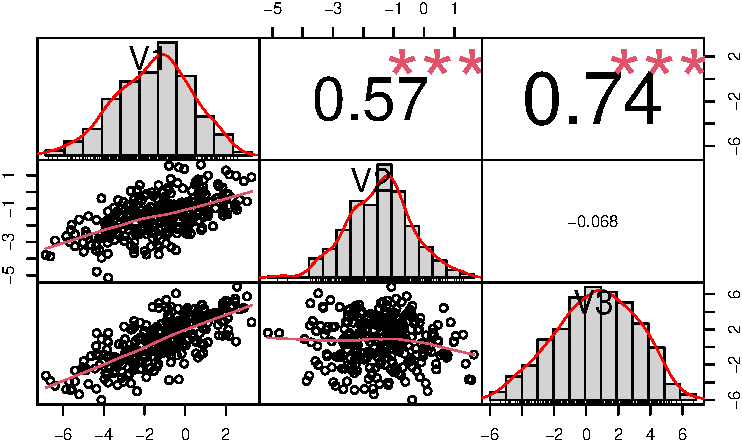
\includegraphics{lista-6_files/figure-pdf/fig-linear1-1.pdf}

}

\caption{\label{fig-linear1}Correlações e histogramas das variáveis
explicativas.}

\end{figure}%

\begin{Shaded}
\begin{Highlighting}[]
\FunctionTok{with}\NormalTok{(train\_linear, }\FunctionTok{pairs}\NormalTok{(}
\NormalTok{  train\_linear }\SpecialCharTok{\%\textgreater{}\%}\NormalTok{ dplyr}\SpecialCharTok{::}\FunctionTok{select}\NormalTok{(V1}\SpecialCharTok{:}\NormalTok{V3),}
  \AttributeTok{col =} \FunctionTok{with}\NormalTok{(train\_linear, }\FunctionTok{c}\NormalTok{(}\AttributeTok{A =} \StringTok{"black"}\NormalTok{, }\AttributeTok{B =} \StringTok{"pink"}\NormalTok{)[Grupo]),}
  \AttributeTok{upper.panel =} \ControlFlowTok{function}\NormalTok{(...) \{\}}
\NormalTok{))}
\end{Highlighting}
\end{Shaded}

\begin{figure}[H]

\centering{

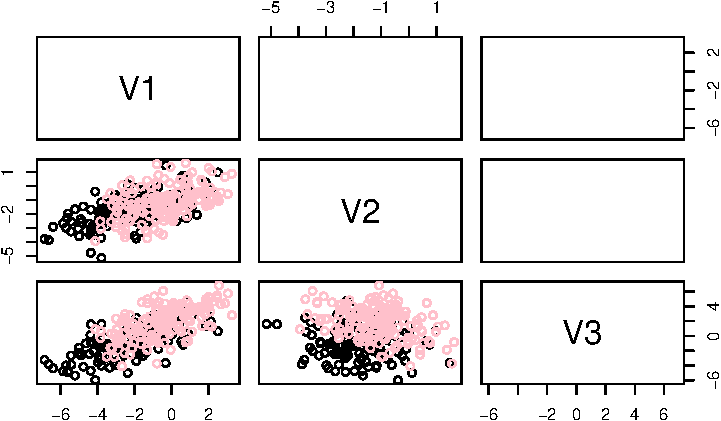
\includegraphics{lista-6_files/figure-pdf/fig-linear2-1.pdf}

}

\caption{\label{fig-linear2}Gráficos de dispersão das variáveis
explicativas com marcadores por classes linearmente separáveis.}

\end{figure}%

~

Como esperado, muitos dados estão espalhados e em regiões sobrepostas,
com várias delas correlacionadas, o que dá indícios da possibilidade de
rotações.

A biblioteca \texttt{MASS} possui um comando pré-implementado que ajusta
um LDA.

A principal forma de se definir o modelo é:

\begin{itemize}
\item
  \texttt{formula}: Sintaxe de fórmula análoga a qualquer outra
  modelagem em R.
\item
  \texttt{data}: Dados a partir dos quais os coeficientes da fórmula
  serão ajustados. O argumento é opcional, caso cada elemento da fórmula
  esteja individualmente definido.
\end{itemize}

Existe também uma forma alternativa não muito usual:

\begin{itemize}
\item
  \texttt{x}: Conjunto de dados com variáveis explicativas;
\item
  \texttt{grouping}: Variável resposta contendo as categorias a serem
  previstas.
\end{itemize}

O método também permite selecionar as probabilidades de cada classe,
métodos de estimação e se o modelo será treinado com validação cruzada
ou não. Por padrão, ele não utiliza validação cruzada.

Ajustando três LDAs com apenas duas variáveis cada (e todos os
argumentos default), obtemos:

~

\begin{Shaded}
\begin{Highlighting}[]
\NormalTok{incomplete\_ldas }\OtherTok{\textless{}{-}} \FunctionTok{list}\NormalTok{(}
  \AttributeTok{V1V2 =} \FunctionTok{lda}\NormalTok{(Grupo }\SpecialCharTok{\textasciitilde{}}\NormalTok{ V1 }\SpecialCharTok{+}\NormalTok{ V2, train\_linear),}
  \AttributeTok{V2V3 =} \FunctionTok{lda}\NormalTok{(Grupo }\SpecialCharTok{\textasciitilde{}}\NormalTok{ V2 }\SpecialCharTok{+}\NormalTok{ V3, train\_linear),}
  \AttributeTok{V1V3 =} \FunctionTok{lda}\NormalTok{(Grupo }\SpecialCharTok{\textasciitilde{}}\NormalTok{ V1 }\SpecialCharTok{+}\NormalTok{ V3, train\_linear)}
\NormalTok{)}

\FunctionTok{with}\NormalTok{(incomplete\_ldas, V1V2)}
\end{Highlighting}
\end{Shaded}

\begin{verbatim}
Call:
lda(Grupo ~ V1 + V2, data = train_linear)

Prior probabilities of groups:
        A         B 
0.4486301 0.5513699 

Group means:
          V1        V2
A -2.1953259 -1.737232
B -0.4581957 -1.152510

Coefficients of linear discriminants:
          LD1
V1 0.54269666
V2 0.01850085
\end{verbatim}

~

O resultado do método mostra a probabilidade de ocorrência de cada grupo
(quando não definido manualmente, é utilizada a probabilidade nos
dados), assim como a média e os coeficientes dos discriminantes. É
possível plotar os resultados assim:

\begin{figure}[H]

\begin{minipage}{0.50\linewidth}

\centering{

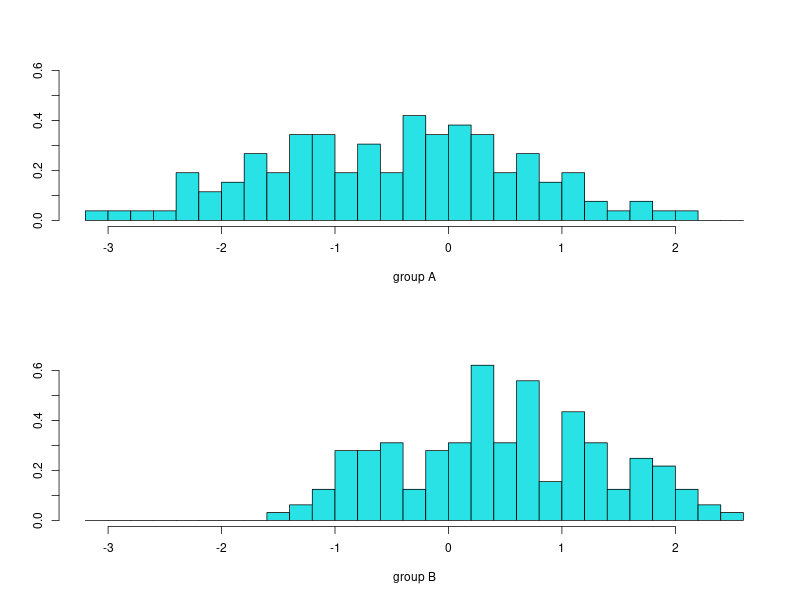
\includegraphics{plot1.png}

}

\subcaption{\label{fig-v1v2}Grupo \textasciitilde{} V1 + V2}

\end{minipage}%
%
\begin{minipage}{0.50\linewidth}

\centering{

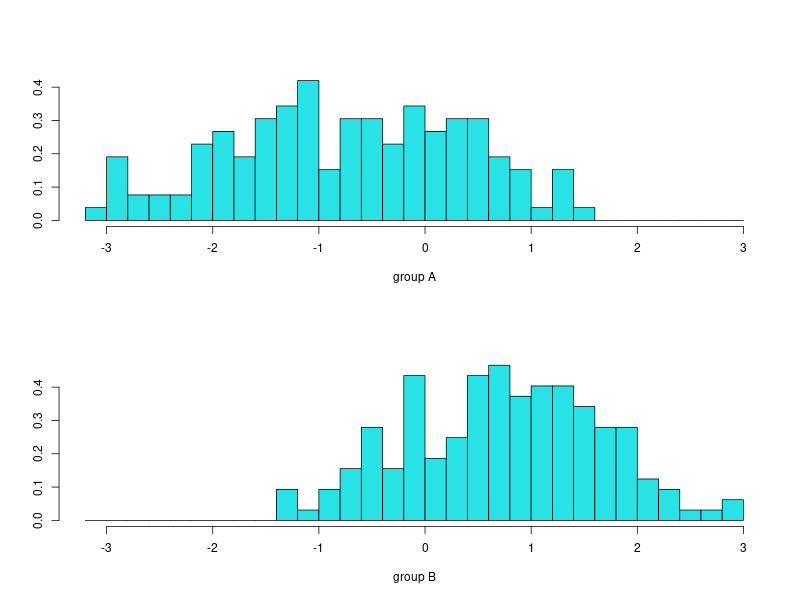
\includegraphics{plot2.png}

}

\subcaption{\label{fig-v2v3}Grupo \textasciitilde{} V2 + V3}

\end{minipage}%
\newline
\begin{minipage}{0.50\linewidth}

\centering{

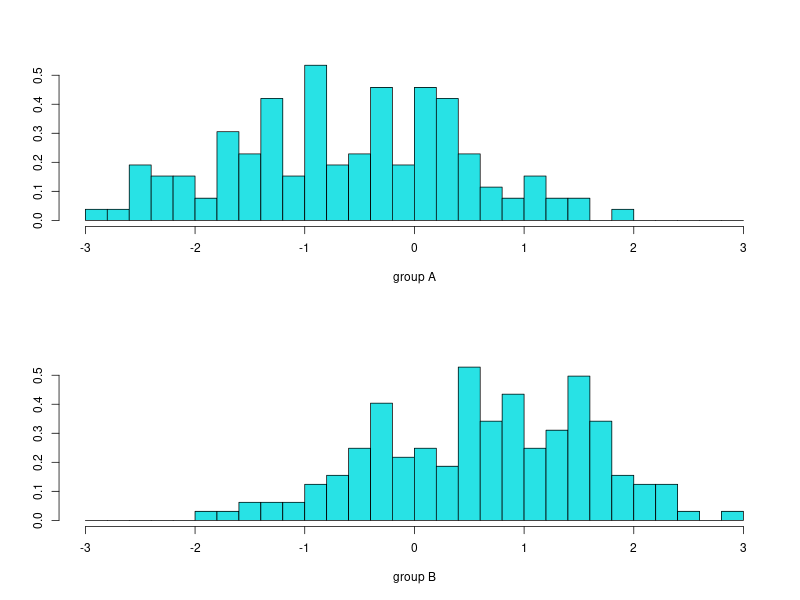
\includegraphics{plot3.png}

}

\subcaption{\label{fig-v1v3}Grupo \textasciitilde{} V1 + V3}

\end{minipage}%

\caption{\label{fig-elephants}Histogramas dos LDAs ajustados com duas
variáveis explicativas.}

\end{figure}%

Testando a acurácia com apenas duas variáveis explicativas, se obtém:

~

\begin{Shaded}
\begin{Highlighting}[]
\ControlFlowTok{for}\NormalTok{ (mdl }\ControlFlowTok{in} \FunctionTok{names}\NormalTok{(incomplete\_ldas)) }\FunctionTok{paste}\NormalTok{(}
  \StringTok{"Acurácia:"}\NormalTok{, mdl, }\FunctionTok{accuracy}\NormalTok{(}
\NormalTok{    incomplete\_ldas[[mdl]],}
\NormalTok{    test\_linear,}
    \FunctionTok{with}\NormalTok{(test\_linear, Grupo)), }\StringTok{\textquotesingle{}}\SpecialCharTok{\textbackslash{}n}\StringTok{\textquotesingle{}}
\NormalTok{) }\SpecialCharTok{\%\textgreater{}\%}
  \FunctionTok{cat}\NormalTok{()}
\end{Highlighting}
\end{Shaded}

\begin{verbatim}
Acurácia: V1V2 0.589 
Acurácia: V2V3 0.671 
Acurácia: V1V3 0.644 
\end{verbatim}

\begin{Shaded}
\begin{Highlighting}[]
\NormalTok{(lda\_full }\OtherTok{\textless{}{-}} \FunctionTok{lda}\NormalTok{(Grupo }\SpecialCharTok{\textasciitilde{}}\NormalTok{ V1 }\SpecialCharTok{+}\NormalTok{ V2 }\SpecialCharTok{+}\NormalTok{ V3, train\_linear))}
\end{Highlighting}
\end{Shaded}

\begin{verbatim}
Call:
lda(Grupo ~ V1 + V2 + V3, data = train_linear)

Prior probabilities of groups:
        A         B 
0.4486301 0.5513699 

Group means:
          V1        V2         V3
A -2.1953259 -1.737232 -0.7887385
B -0.4581957 -1.152510  1.8861528

Coefficients of linear discriminants:
         LD1
V1 -1.808266
V2  2.441663
V3  1.543961
\end{verbatim}

\begin{Shaded}
\begin{Highlighting}[]
\FunctionTok{paste}\NormalTok{(}\StringTok{"Acurácia:"}\NormalTok{, }\FunctionTok{accuracy}\NormalTok{(lda\_full, test\_linear, }\FunctionTok{with}\NormalTok{(test\_linear, Grupo))) }\SpecialCharTok{\%\textgreater{}\%}
  \FunctionTok{cat}\NormalTok{()}
\end{Highlighting}
\end{Shaded}

\begin{verbatim}
Acurácia: 0.904
\end{verbatim}

~

Com apenas duas variáveis, nenhum dos classificadores atinge acurácia
maior que 70\%. Utilizando as três, o resultado ultrapassa 90\% de
acurácia.

Ajustando um modelo QDA para os mesmos dados (que não é o uso mais
adequado da técnica, uma vez que as variâncias são iguais e eles são
linearmente separáveis), o resultado é:

~

\begin{Shaded}
\begin{Highlighting}[]
\FunctionTok{paste}\NormalTok{(}\StringTok{"Acurácia:"}\NormalTok{, }\FunctionTok{accuracy}\NormalTok{(}
  \FunctionTok{qda}\NormalTok{(Grupo }\SpecialCharTok{\textasciitilde{}}\NormalTok{ V1 }\SpecialCharTok{+}\NormalTok{ V2 }\SpecialCharTok{+}\NormalTok{ V3, train\_linear),}
\NormalTok{  test\_linear, }\FunctionTok{with}\NormalTok{(test\_linear, Grupo))}
\NormalTok{) }\SpecialCharTok{\%\textgreater{}\%}
  \FunctionTok{cat}\NormalTok{()}
\end{Highlighting}
\end{Shaded}

\begin{verbatim}
Acurácia: 0.89
\end{verbatim}

~

Que é um resultado inferior ao modelo LDA completo.

Para uma implementação do QDA, os grupos serão modificados a partir dos
mesmos dados, forçando que a separação não-linear seja mais adequada que
uma separação linear. Os resultados são expostos a seguir.

~

\begin{Shaded}
\begin{Highlighting}[]
\NormalTok{nonlinear }\OtherTok{\textless{}{-}}\NormalTok{ linear }\SpecialCharTok{\%\textgreater{}\%}
  \FunctionTok{mutate}\NormalTok{(}
    \AttributeTok{Grupo =} \FunctionTok{ifelse}\NormalTok{(}
\NormalTok{      (}
        \FunctionTok{abs}\NormalTok{(V1 }\SpecialCharTok{\^{}} \DecValTok{2} \SpecialCharTok{*} \FunctionTok{rgamma}\NormalTok{(}\FunctionTok{n}\NormalTok{(), }\DecValTok{3}\NormalTok{) }\SpecialCharTok{*}\NormalTok{ V3 }\SpecialCharTok{{-}}\NormalTok{ V2 }\SpecialCharTok{\^{}} \DecValTok{3}\NormalTok{) }\SpecialCharTok{\textgreater{}}
          \FunctionTok{mean}\NormalTok{(}\SpecialCharTok{{-}}\NormalTok{V1 }\SpecialCharTok{+}\NormalTok{ V2 }\SpecialCharTok{{-}}\NormalTok{ V3) }\SpecialCharTok{/} \DecValTok{2} \SpecialCharTok{+} \FunctionTok{rnorm}\NormalTok{(}\FunctionTok{n}\NormalTok{(), }\DecValTok{10}\NormalTok{)}
\NormalTok{      ),}
      \StringTok{"A"}\NormalTok{, }\StringTok{"B"}
\NormalTok{    )}
\NormalTok{  )}

\NormalTok{train\_nonlinear }\OtherTok{\textless{}{-}}\NormalTok{ nonlinear }\SpecialCharTok{\%\textgreater{}\%}
  \FunctionTok{filter}\NormalTok{(rows\_train)}

\NormalTok{test\_nonlinear }\OtherTok{\textless{}{-}}\NormalTok{ nonlinear }\SpecialCharTok{\%\textgreater{}\%}
  \FunctionTok{filter}\NormalTok{(}\SpecialCharTok{!}\NormalTok{rows\_train)}

\FunctionTok{with}\NormalTok{(train\_nonlinear, }\FunctionTok{pairs}\NormalTok{(}
\NormalTok{  train\_nonlinear }\SpecialCharTok{\%\textgreater{}\%}\NormalTok{ dplyr}\SpecialCharTok{::}\FunctionTok{select}\NormalTok{(V1}\SpecialCharTok{:}\NormalTok{V3),}
  \AttributeTok{col =} \FunctionTok{with}\NormalTok{(train\_nonlinear, }\FunctionTok{c}\NormalTok{(}\AttributeTok{A =} \StringTok{"black"}\NormalTok{, }\AttributeTok{B =} \StringTok{"pink"}\NormalTok{)[Grupo]),}
  \AttributeTok{upper.panel =} \ControlFlowTok{function}\NormalTok{(...) \{\}}
\NormalTok{))}
\end{Highlighting}
\end{Shaded}

\begin{figure}[H]

\centering{

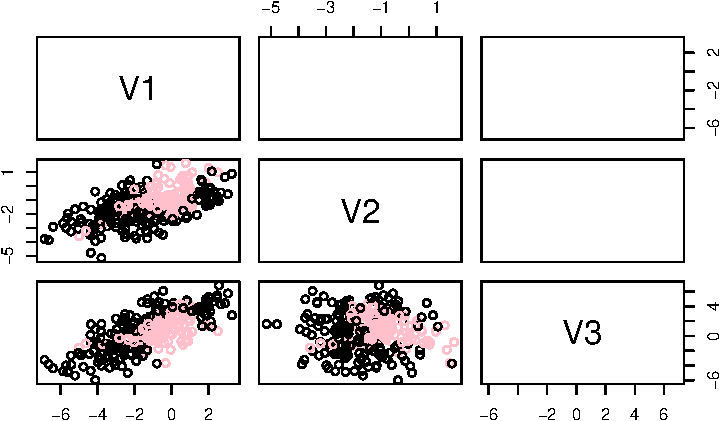
\includegraphics{lista-6_files/figure-pdf/fig-nonlinear-1.pdf}

}

\caption{\label{fig-nonlinear}Gráficos de dispersão das variáveis
explicativas com marcadores por classes não-linearmente separáveis.}

\end{figure}%

~

Se observa, em todas as variáveis, regiões curvadas onde seria possível
estabelecer limites de classificação. Ainda há algum nível de confusão
entre as regiões, de forma que a separçaão não é perfeita.

Ajustando um QDA com as variáveis nessa estrutura, obtemos:

~

\begin{Shaded}
\begin{Highlighting}[]
\NormalTok{incomplete\_qdas }\OtherTok{\textless{}{-}} \FunctionTok{list}\NormalTok{(}
  \AttributeTok{V1V2 =} \FunctionTok{qda}\NormalTok{(Grupo }\SpecialCharTok{\textasciitilde{}}\NormalTok{ V1 }\SpecialCharTok{+}\NormalTok{ V2, train\_linear),}
  \AttributeTok{V2V3 =} \FunctionTok{qda}\NormalTok{(Grupo }\SpecialCharTok{\textasciitilde{}}\NormalTok{ V2 }\SpecialCharTok{+}\NormalTok{ V3, train\_linear),}
  \AttributeTok{V1V3 =} \FunctionTok{qda}\NormalTok{(Grupo }\SpecialCharTok{\textasciitilde{}}\NormalTok{ V1 }\SpecialCharTok{+}\NormalTok{ V3, train\_linear)}
\NormalTok{)}

\ControlFlowTok{for}\NormalTok{ (mdl }\ControlFlowTok{in} \FunctionTok{names}\NormalTok{(incomplete\_qdas)) }\FunctionTok{paste}\NormalTok{(}
  \StringTok{"Acurácia:"}\NormalTok{, mdl, }\FunctionTok{accuracy}\NormalTok{(}
\NormalTok{    incomplete\_qdas[[mdl]],}
\NormalTok{    test\_nonlinear,}
    \FunctionTok{with}\NormalTok{(test\_nonlinear, Grupo)), }\StringTok{\textquotesingle{}}\SpecialCharTok{\textbackslash{}n}\StringTok{\textquotesingle{}}
\NormalTok{) }\SpecialCharTok{\%\textgreater{}\%}
  \FunctionTok{cat}\NormalTok{()}
\end{Highlighting}
\end{Shaded}

\begin{verbatim}
Acurácia: V1V2 0.795 
Acurácia: V2V3 0.767 
Acurácia: V1V3 0.671 
\end{verbatim}

\begin{Shaded}
\begin{Highlighting}[]
\FunctionTok{paste}\NormalTok{(}
  \StringTok{"Acurácia:"}\NormalTok{, }\FunctionTok{accuracy}\NormalTok{(}
    \FunctionTok{qda}\NormalTok{(Grupo }\SpecialCharTok{\textasciitilde{}}\NormalTok{ V1 }\SpecialCharTok{+}\NormalTok{ V2 }\SpecialCharTok{+}\NormalTok{ V3, train\_nonlinear),}
\NormalTok{    test\_nonlinear,}
    \FunctionTok{with}\NormalTok{(test\_nonlinear, Grupo)), }\StringTok{\textquotesingle{}}\SpecialCharTok{\textbackslash{}n}\StringTok{\textquotesingle{}}
\NormalTok{) }\SpecialCharTok{\%\textgreater{}\%}
  \FunctionTok{cat}\NormalTok{()}
\end{Highlighting}
\end{Shaded}

\begin{verbatim}
Acurácia: 0.932 
\end{verbatim}

~

Para estes dados, uma das classificações com duas variáveis (V1 com V2)
já chegou a uma acurácia próxima de 80\%. Utilizando as três, mais de
93\% dos pontos são classificados corretamente.

Ajustando um LDA para os dados não-lineares, a título de comparação, se
obtém:

~

\begin{Shaded}
\begin{Highlighting}[]
\FunctionTok{accuracy}\NormalTok{(}
  \FunctionTok{lda}\NormalTok{(Grupo }\SpecialCharTok{\textasciitilde{}}\NormalTok{ V1 }\SpecialCharTok{+}\NormalTok{ V2 }\SpecialCharTok{+}\NormalTok{ V3, train\_nonlinear),}
\NormalTok{  test\_nonlinear, }\FunctionTok{with}\NormalTok{(test\_nonlinear, Grupo)}
\NormalTok{)}
\end{Highlighting}
\end{Shaded}

\begin{verbatim}
[1] 0.767
\end{verbatim}

~

Que é uma precisão mais baixa que a precisão do QDA, como esperado pelo
fato de a aplicação LDA não ser o uso mais adequado do método para esses
dados.

Apesar disso, mesmo não sendo o uso mais adequado, o ajuste LDA ainda
acertou mais de 75\% das classificações.



\end{document}
